\documentclass{article}
\usepackage{amsfonts, amsthm, amsmath, amssymb, mathtools, ulem, mathrsfs, physics, esint, siunitx, tikz-cd}
\usepackage{pdfpages, fullpage, color, microtype, cancel, textcomp, markdown, hyperref, graphicx}
\usepackage{enumitem}
\usepackage{algorithm}
\usepackage{algpseudocode}
\graphicspath{{./images/}}
\usepackage[english]{babel}
\usepackage[autostyle, english=american]{csquotes}
\MakeOuterQuote{"}
\usepackage{xparse}
\usepackage{tikz}

\usepackage{calligra}
\DeclareMathAlphabet{\mathcalligra}{T1}{calligra}{m}{n}
\DeclareFontShape{T1}{calligra}{m}{n}{<->s*[2.2]callig15}{}
\newcommand{\script}[1]{\ensuremath{\mathcalligra{#1}}}
\newcommand{\scr}{\script r}

% fonts
\def\mbb#1{\mathbb{#1}}
\def\mfk#1{\mathfrak{#1}}
\def\mbf#1{\mathbf{#1}}
\def\tbf#1{\textbf{#1}}

% common bold letters
\def\bP{\mbb{P}}
\def\bC{\mbb{C}}
\def\bH{\mbb{H}}
\def\bI{\mbb{I}}
\def\bR{\mbb{R}}
\def\bQ{\mbb{Q}}
\def\bZ{\mbb{Z}}
\def\bN{\mbb{N}}

% brackets
\newcommand{\br}[1]{\left(#1\right)}
\newcommand{\sbr}[1]{\left[#1\right]}
\newcommand{\brc}[1]{\left\{#1\right\}}
\newcommand{\lbr}[1]{\left\langle#1\right\rangle}

% vectors
\renewcommand{\i}{\hat{\imath}}
\renewcommand{\j}{\hat{\jmath}}
\renewcommand{\k}{\hat{k}}
\newcommand{\proj}[2]{\text{proj}_{#2}\br{#1}}
\newcommand{\m}[2][b]{\begin{#1matrix}#2\end{#1matrix}}
\newcommand{\arr}[3][\sbr]{#1{\begin{array}{#2}#3\end{array}}}

% misc
\NewDocumentCommand{\seq}{O{n} O{1} O{\infty} m}{\br{#4}_{{#1}={#2}}^{#3}}
\NewDocumentCommand{\app}{O{x} O{\infty}}{\xrightarrow{#1\to#2}}
\newcommand{\sm}{\setminus}
\newcommand{\sse}{\subseteq}
\renewcommand{\ss}{\subset}
\newcommand{\vn}{\varnothing}
\newcommand{\lc}{\epsilon_{ijk}}
\newcommand{\ep}{\epsilon}
\newcommand{\vp}{\varphi}
\renewcommand{\th}{\theta}
\newcommand{\cjg}[1]{\overline{#1}}
\newcommand{\inv}{^{-1}}
\DeclareMathOperator{\im}{im}
\DeclareMathOperator{\id}{id}
\newcommand{\ans}{\tbf{Ans. }}
\newcommand{\pf}{\tbf{Pf. }}
\newcommand{\imp}{\implies}
\newcommand{\impleft}{\reflectbox{$\implies$}}
\newcommand{\ck}{\frac1{4\pi\ep_0}}
\newcommand{\ckb}{4\pi\ep_0}
\newcommand{\sto}{\longrightarrow}
\DeclareMathOperator{\cl}{cl}
\DeclareMathOperator{\intt}{int}
\DeclareMathOperator{\bd}{bd}
\DeclareMathOperator{\Span}{span}
\newcommand{\floor}[1]{\left\lfloor#1\right\rfloor}
\newcommand{\ceil}[1]{\left\lceil#1\right\rceil}
\newcommand{\fxn}[5]{#1:\begin{array}{rcl}#2&\longrightarrow & #3\\[-0.5mm]#4&\longmapsto &#5\end{array}}
\newcommand{\sep}[1][.5cm]{\vspace{#1}}
\DeclareMathOperator{\card}{card}
\renewcommand{\ip}[2]{\lbr{#1,#2}}
\renewcommand{\bar}{\overline}
\DeclareMathOperator{\cis}{cis}
\DeclareMathOperator{\Arg}{Arg}
\DeclareMathOperator{\diag}{diag}
\newcommand{\ptl}{\partial}

% title
\title{Scientific Computing HW 11}
\author{Ryan Chen}
%\date{\today}
\setlength{\parindent}{0pt}


\begin{document}
	
\maketitle



\tbf{Problem 1.}

\begin{enumerate}[label=(\alph*)]
	
\item The form of solution is
$$u(x,t) = \frac12[\vp(x+at)+\vp(x-at)] + \frac{1}{2a}\int_{x-at}^{x+at}\psi(s)ds$$
First find $u_{tt}$.
$$u_t = \frac12[\vp'(x+at)\cdot a+\vp'(x-at)\cdot(-a)] + \frac{1}{2a}[\psi(x+at)\cdot a-\psi(x-at)\cdot(-a)]$$
$$= \frac{a}{2}[\vp'(x+at)-\vp'(x-at)] + \frac12[\psi(x+at)+\psi(x-at)]$$
$$u_{tt} = \frac{a^2}{2}[\vp''(x+at)+\vp''(x-at)] + \frac a2[\psi'(x+at)-\psi'(x-at)]$$
Then find $a^2u_{xx}$ and see that it equals $u_{tt}$, hence $u$ solves the PDE.
$$u_x = \frac12[\vp'(x+at)+\vp'(x-at)] + \frac{1}{2a}[\psi(x+at)-\psi(x-at)]$$
$$u_{xx} = \frac12[\vp''(x+at)+\vp''(x-at)] + \frac{1}{2a}[\psi'(x+at)-\psi'(x-at)]$$
$$a^2u_{xx} = \frac{a^2}{2}[\vp''(x+at)+\vp''(x-at)] + \frac{a}{2}[\psi'(x+at)-\psi'(x-at)] = u_{tt}$$


\item Consider the form of solution
$$u(x,t) = \frac12[\vp(x+at)+\vp(x-at)] + \frac{1}{2a}\int_{x-at}^{x+at}\psi(s)ds$$

To find the domain of influence of a point $x_0$, note that $u(x,t)$ depends on the initial conditions at $x_0$ iff the integral in the second term depends on $\psi(x_0)$, which holds iff $x-at\le x\le x+at$. Then we have
$$x-at \le x \le x+at
\iff -at \le x_0-x \le at
\iff at \ge x-x_0 \ge -at
\iff x_0+at \ge x \ge x_0-at$$
Thus the domain of influence of $x_0$ is the region bounded by the lines $x=x_0-at$ and $x=x_0+at$.

\begin{center}
	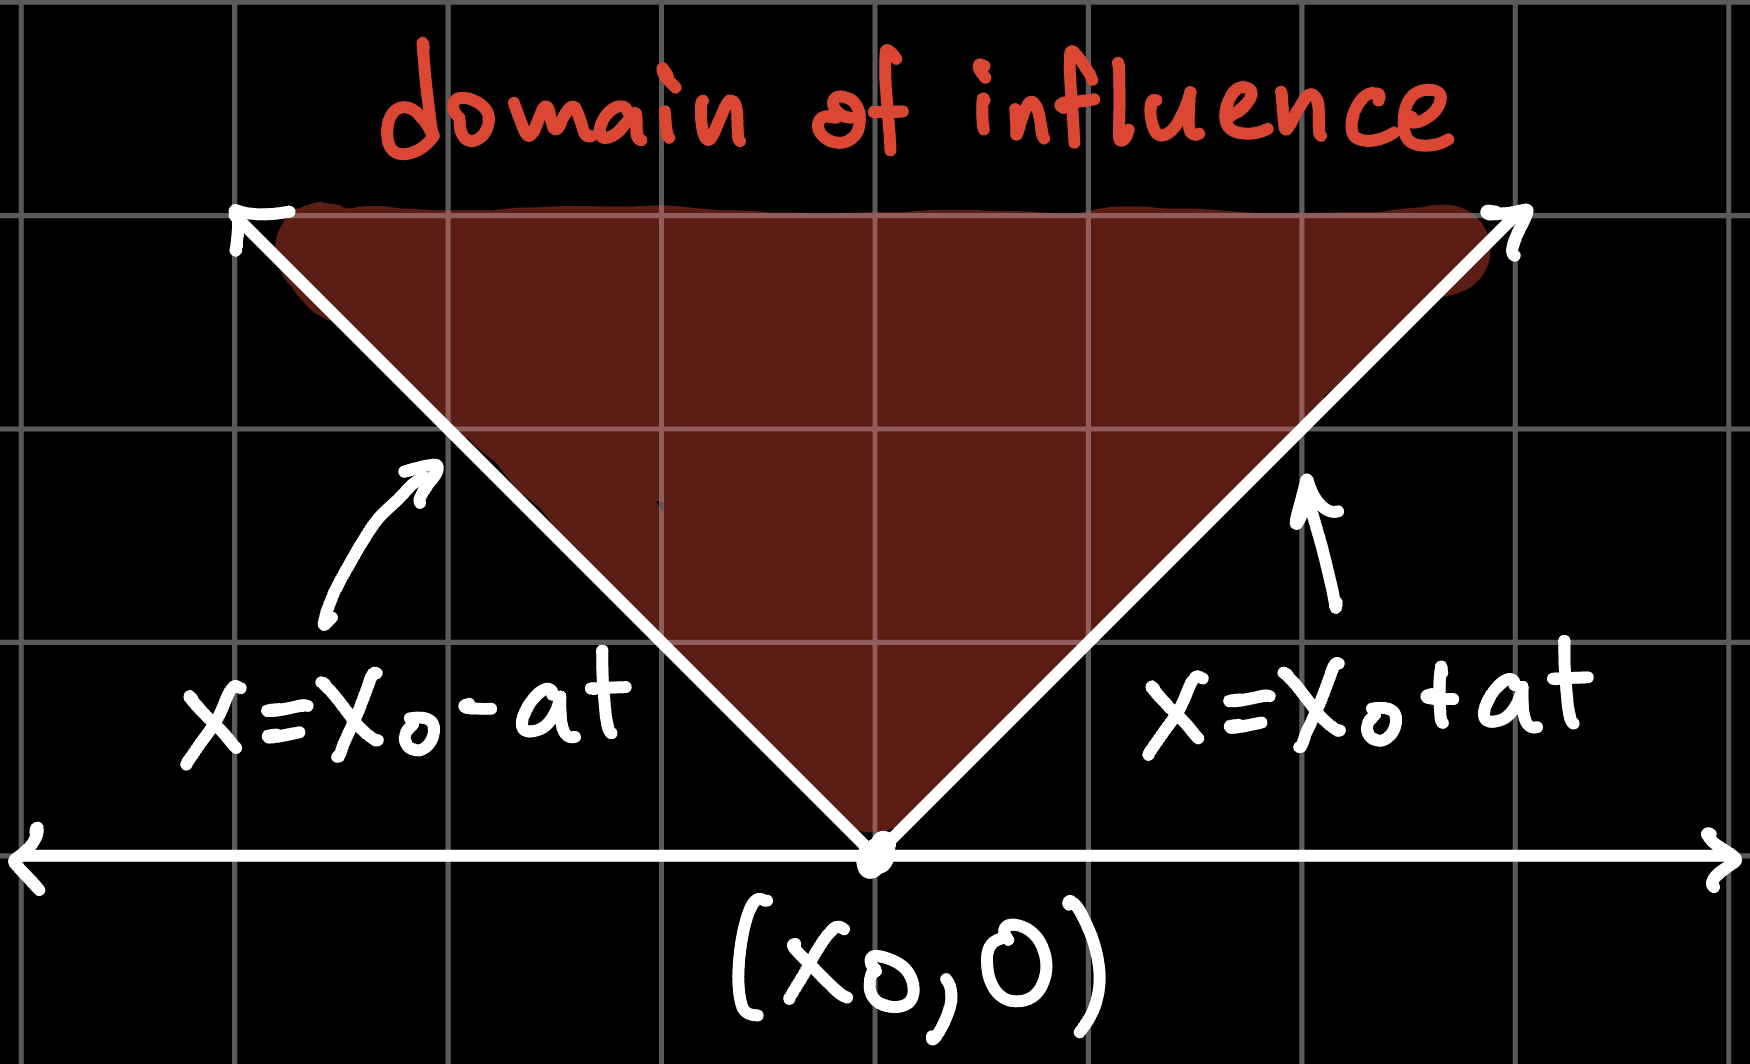
\includegraphics[scale=.1]{hw11 doi}
\end{center}

Now to find the domain of dependence of a point $(x,t)$, note that $u(x,t)$ depends precisely on the values of $\vp$ at $x\pm at$ and the values of $\psi$ on $[x-at,x+at]$. Thus the domain of dependence of $(x,t)$ is the line segment $\brc{(s,0):x-at\le s\le x+at}$.

\begin{center}
	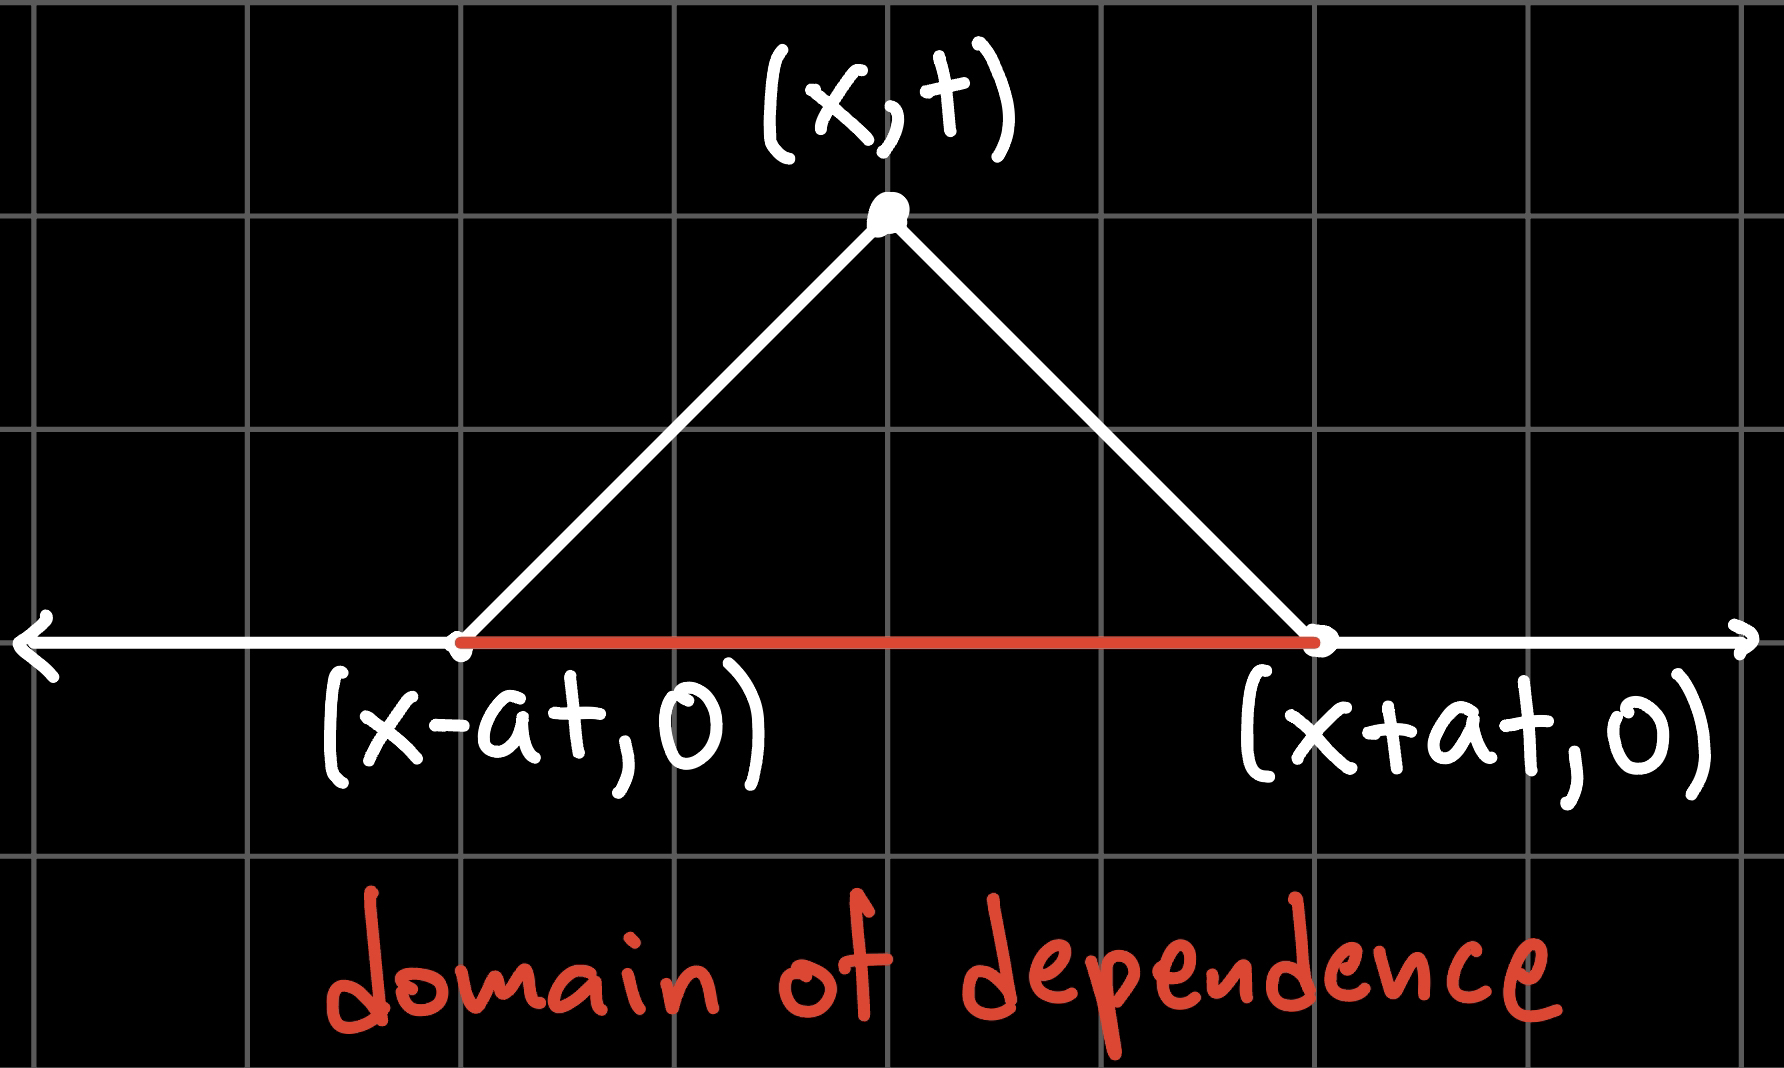
\includegraphics[scale=.1]{hw11 dod}
\end{center}


\item We see that
$$w := \m{u_t \\ u_x}
\imp w_x = \m{u_{tx} \\ u_{xx}}$$
so that
$$w_t = \m{u_{tt} \\ u_{xt}}
= \m{0u_{tx}+a^2u_{xx} \\ 1u_{tx}+0u_{xx}}
= \underbrace{\m{0 & a^2 \\ 1 & 0}}_{=:A}\m{u_{tx} \\ u_{xx}}
= Aw_x$$
Then
$$u_x\eval_{t=0} = \frac12[\vp'(x)+\vp'(x)] + \frac{1}{2a}[\psi(x)-\psi(x)]
= \vp'(x)$$
so that the initial condition for $w$ is
$$w\eval_{t=0} = \m{u_t\eval_{t=0} \\ u_x\eval_{t=0}}
= \m{\psi(x) \\ \vp'(x)}$$


\item The eigenvalues of $A$ are
$$0 = \det(A-\lambda I)
= \m[v]{-\lambda & a^2 \\ 1 & -\lambda}
= \lambda^2 - a^2
= (\lambda-a)(\lambda+a)
\imp \lambda_1 = a,~\lambda_2 = -a$$
Eigenvectors $v_1,v_2$ of $A$ are
$$A-\lambda_1I = \m{-a & a^2 \\ 1 & -a}
\imp v_1 = \m{a \\ 1}$$
$$A-\lambda_2I = \m{a & a^2 \\ 1 & a}
\imp v_2 = \m{-a \\ 1}$$
Diagonalizing $A$,
$$A = C\Lambda C\inv,
\quad C := [v_1,v_2] = \m{a & -a \\ 1 & 1},
\quad \Lambda := \diag(\lambda_1,\lambda_2) = \diag(a,-a)$$

Changing variable, we obtain independent PDEs.
$$y := C\inv w = \m{\xi \\ \eta}
\imp w = Cy
\imp w_t = Cy_t,
~w_x = Cy_x$$
$$\imp 0 = w_t - Aw_x
= Cy_t - C\Lambda C\inv Cy_x
= C(y_t-\Lambda y_x)
\imp y_t - \Lambda y_x = 0
\imp y_t = \Lambda y_x$$
$$\imp \xi_t = a\xi_x,
~\eta_t = -a\eta_x$$

First find $C\inv$.
$$\det C = \m[v]{a & -a \\ 1 & 1}
= 2a
\imp C\inv = \frac{1}{2a}\m{1 & a \\ -1 & a}$$
Then we find the initial condition for $y$, i.e. the initial conditions for $\xi,\eta$.
$$\m{\psi(x) \\ \vp'(x)} = w\eval_{t=0} = Cy\eval_{t=0}
\imp y\eval_{t=0} = C\inv\m{\psi(x) \\ \vp'(x)}
= \frac{1}{2a}\m{\psi(x)+a\vp'(x) \\ -\psi(x)+a\vp'(x)}$$


\item Code: \url{https://github.com/RokettoJanpu/Scientific-Computing-2/blob/main/hw11.ipynb}

Lax--Friedrichs:
\begin{center}
	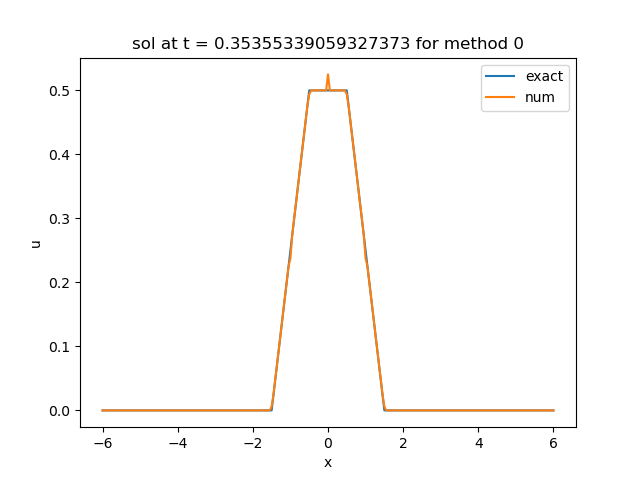
\includegraphics[scale=.3]{hw11 sol n = 10 method 0}
	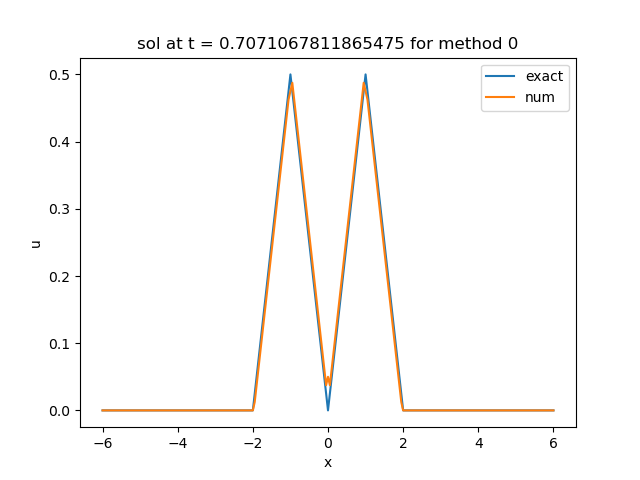
\includegraphics[scale=.3]{hw11 sol n = 20 method 0}
\end{center}
\begin{center}
	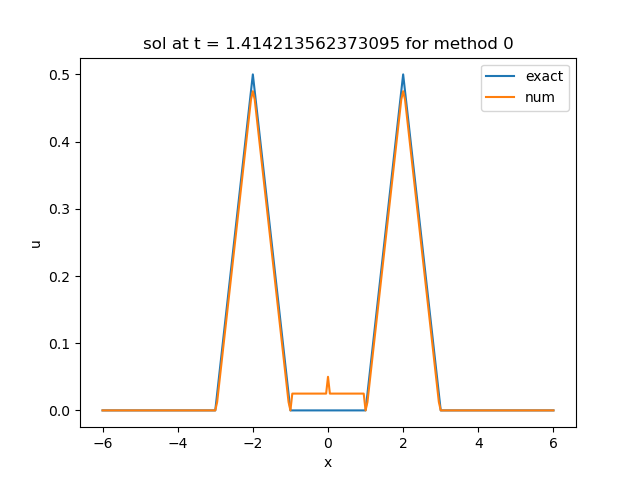
\includegraphics[scale=.3]{hw11 sol n = 40 method 0}
	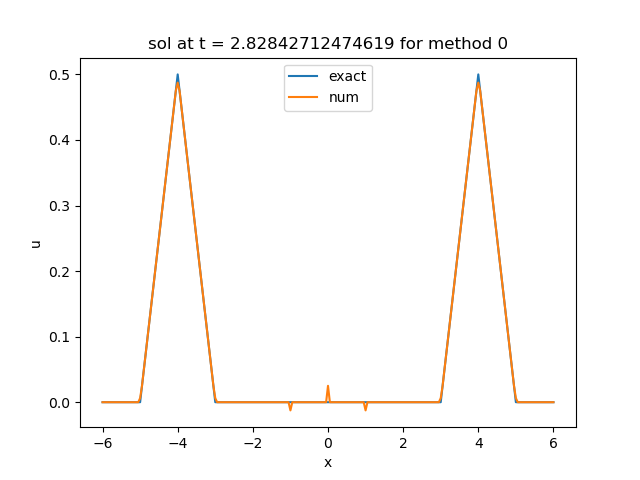
\includegraphics[scale=.3]{hw11 sol n = 80 method 0}
\end{center}

Upwind:
\begin{center}
	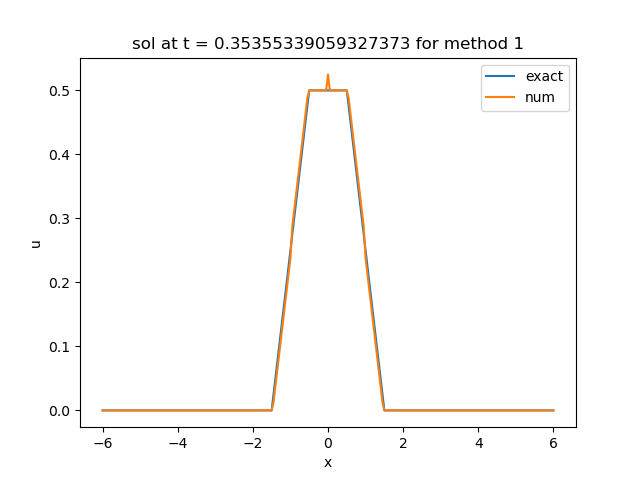
\includegraphics[scale=.3]{hw11 sol n = 10 method 1}
	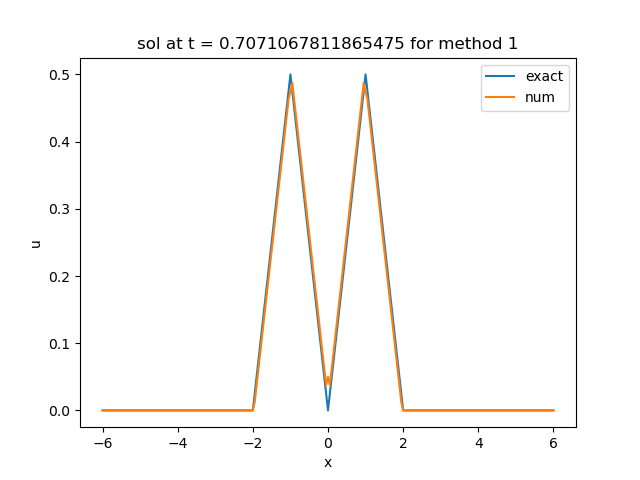
\includegraphics[scale=.3]{hw11 sol n = 20 method 1}
\end{center}
\begin{center}
	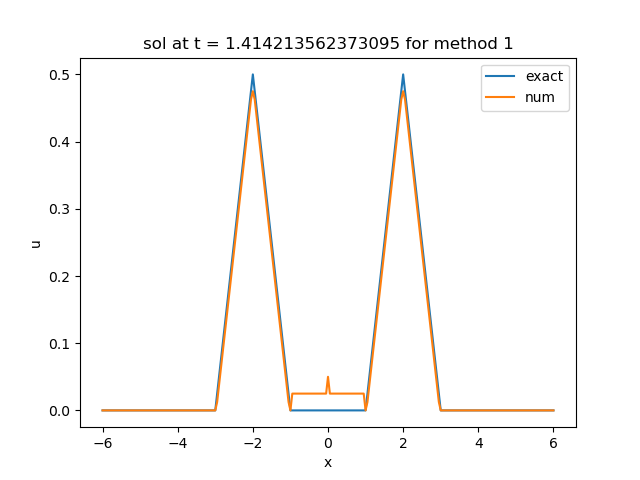
\includegraphics[scale=.3]{hw11 sol n = 40 method 1}
	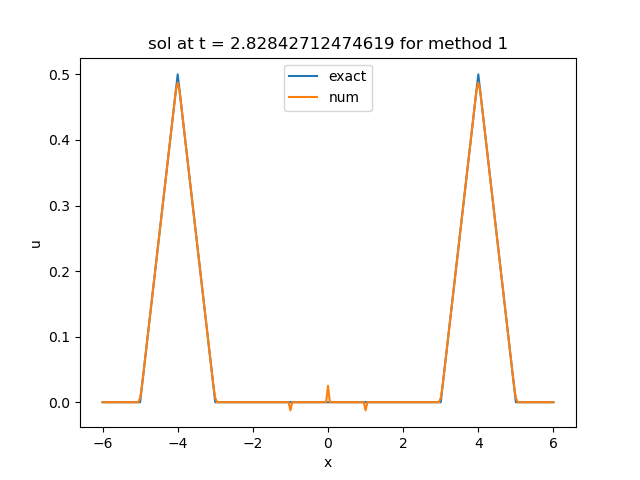
\includegraphics[scale=.3]{hw11 sol n = 80 method 1}
\end{center}

Lax--Wendroff:
\begin{center}
	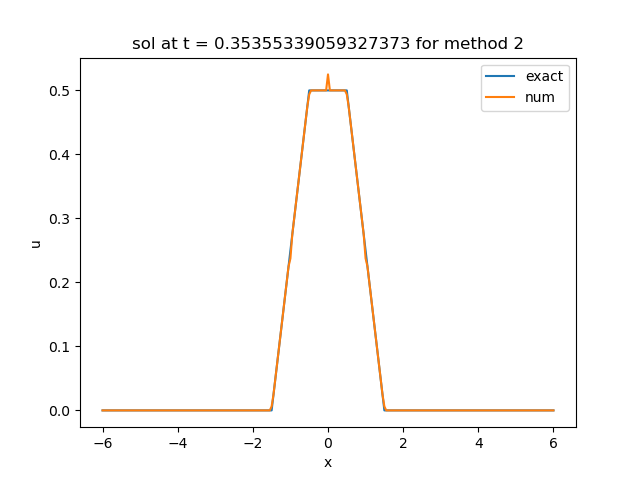
\includegraphics[scale=.3]{hw11 sol n = 10 method 2}
	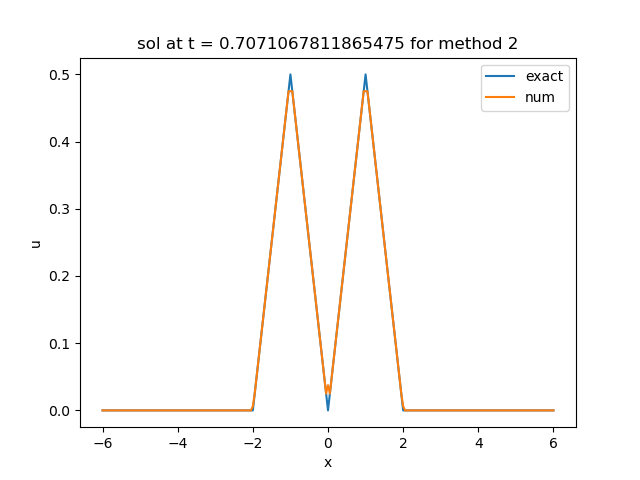
\includegraphics[scale=.3]{hw11 sol n = 20 method 2}
\end{center}
\begin{center}
	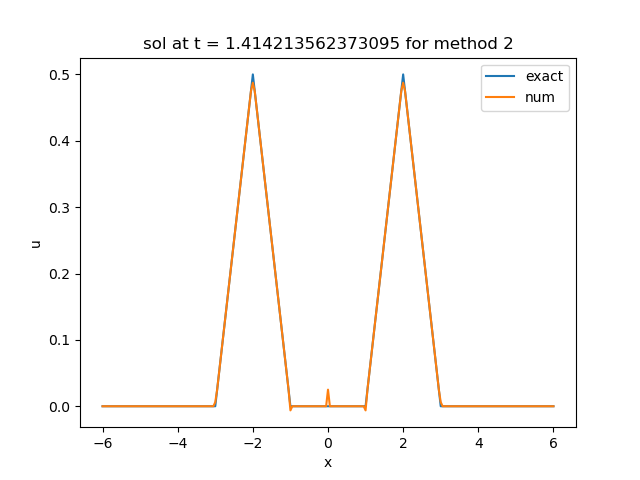
\includegraphics[scale=.3]{hw11 sol n = 40 method 2}
	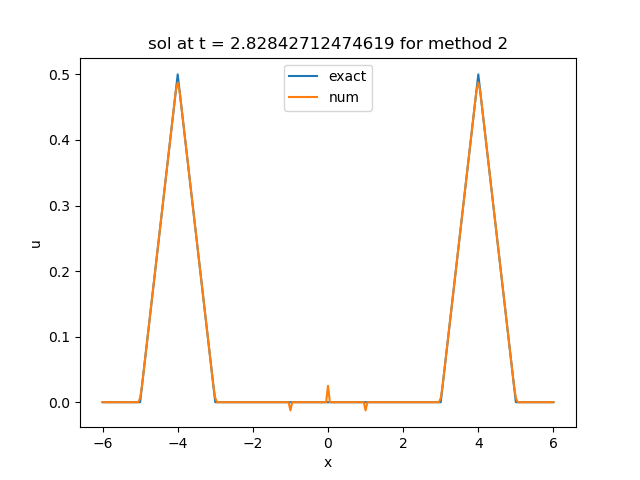
\includegraphics[scale=.3]{hw11 sol n = 80 method 2}
\end{center}

Beam--Warming:
\begin{center}
	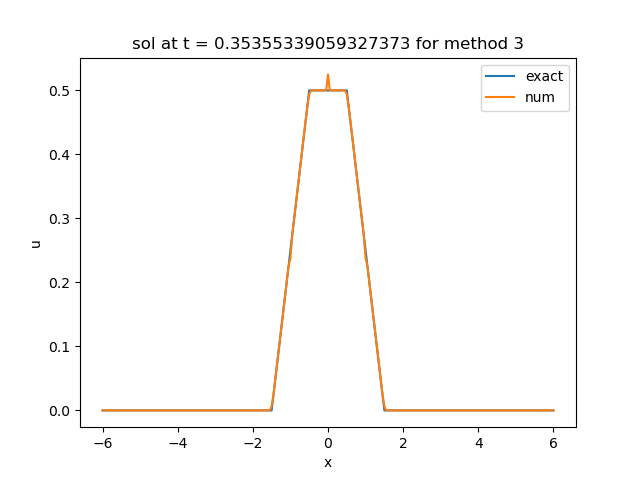
\includegraphics[scale=.3]{hw11 sol n = 10 method 3}
	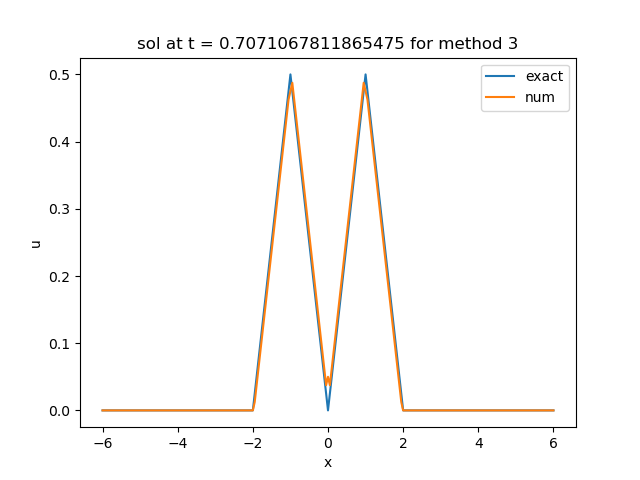
\includegraphics[scale=.3]{hw11 sol n = 20 method 3}
\end{center}
\begin{center}
	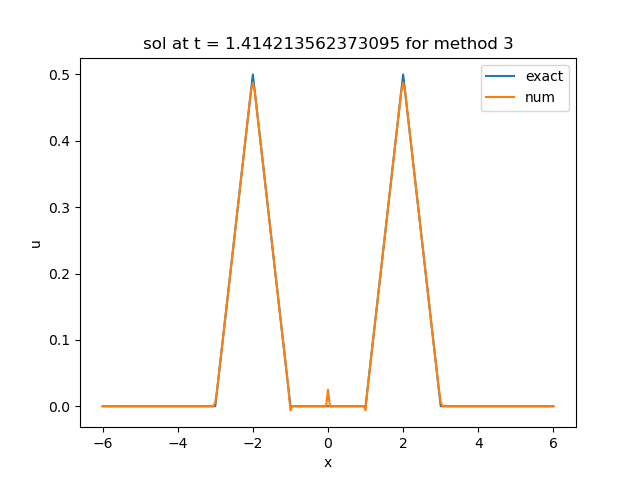
\includegraphics[scale=.3]{hw11 sol n = 40 method 3}
	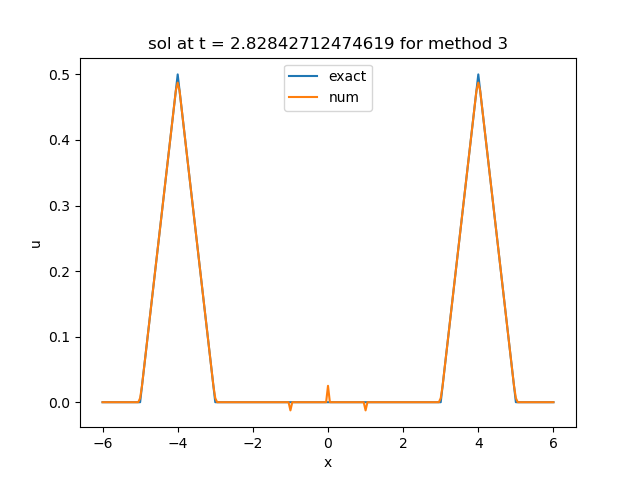
\includegraphics[scale=.3]{hw11 sol n = 80 method 3}
\end{center}

Each scheme is highly accurate in that it computes a solution that essentially coincides with the exact solution, except at finitely many cusps. Stationary cusps arise at points corresponding to cusps of the initial displacement $\vp(x)=\max(1-|x|,0)$, i.e. at $x=0,1,-1$. Cusps that travel along with the solution arise from the form 
$$u(x,t) = \frac12[\vp(x+at)+\vp(x-at)]$$
meaning these cusps occur at $x\pm at=0,1,-1$, i.e. at $x=\mp at,1\mp at,-1\mp at$.
	
\end{enumerate}
\pagebreak



\tbf{Problem 2.}

\begin{enumerate}[label=(\alph*)]
	
\item The LaxFR scheme is
$$u_j^{n+1} = \frac12[u_{j+1}^n + u_{j-1}^n] - \frac12\nu[u_{j+1}^n - u_{j-1}^n]$$
Let $v$ satisfy $v(x_j,t_n)=u_j^n$.
$$v(x,t+k) = \frac12[v(x+h,t) + v(x-h,t)] - \frac12\nu[v(x+h,t) - v(x-h,t)]$$
Taylor expand at $(x,t)$.
\begin{align*}
	v(x,t+k) &= v + kv_t + \frac12k^2v_{tt} + O(k^3)\\
	v(x+h,t) &= v + hv_x + \frac12h^2v_{xx} + \frac16h^3v_{xxx} + O(h^4)\\
	v(x-h,t) &= v - hv_x + \frac12h^2v_{xx} - \frac16h^3v_{xxx} + O(h^4)
\end{align*}
Plug in the expansions.
\begin{align*}
	v + kv_t + \frac12k^2v_{tt} + O(k^3) &= \frac12[2v + h^2v_{xx} + O(h^4)] - \frac12\nu\sbr{2hv_x + \frac26h^3v_{xxx} + O(h^5)}\\
	&= v + \frac12h^2v_{xx} - \nu hv_x + \frac16\nu h^3v_{xxx} + O(h^4)
\end{align*}
Cancel $v$ then divide by $k$.
$$v_t + \frac12kv_{tt} + O(k^2) = \frac12\frac{h^2}{k}v_{xx} - av_x + \frac16\nu \frac{h^3}{k}v_{xxx} + O(h^3)$$
Truncate the $O(h^2)$ and smaller terms.
\begin{align}
	v_t + \frac12kv_{tt} &= \frac12\frac{h^2}{k}v_{xx} - av_x + O(h^2) \nonumber\\
	v_t + av_x &= \frac12\frac{h^2}{k}v_{xx} - \frac12kv_{tt} + O(h^2) \label{eq:2.1}
\end{align}
To express $v_{tt}$ in terms of $v_{xx}$, take $\ptl_t$ and $\ptl_x$ separately.
\begin{align}
	v_{tt} + av_{xt} &= \frac12\frac{h^2}{k}v_{xxt} - \frac12kv_{ttt} + O(h) = O(h) \label{eq:2.2}\\
	v_{tx} + av_{xx} &= \frac12\frac{h^2}{k}v_{xxx} - \frac12kv_{ttx} + O(h) = O(h) \label{eq:2.3}
\end{align}
Take $(\ref{eq:2.2})-a(\ref{eq:2.3})$.
$$v_{tt} - a^2v_{xx} = O(h)
\imp v_{tt} = a^2v_{xx} + O(h)$$
Plug into (\ref{eq:2.1}).
\begin{align*}
	v_t + av_x &= \frac12\frac{h^2}{k}v_{xx} - \frac12k[a^2v_{xx} + O(h)] + O(h^2)\\
	&= \frac12\frac{h^2}{k}\sbr{v_{xx} - \frac12\frac{k^2}{h^2}a^2v_{xx}} + O(h^2)\\
	&= \frac12\frac{h^2}{k}[1-\nu^2]v_{xx} + O(h^2)\\
	&= \frac12\frac{ah}{\nu}[1-\nu^2]v_{xx} + O(h^2)
\end{align*}
Thus the modified equation for LaxFR (first order) is
$$\boxed{v_t + av_x = \frac12\frac{ah}{\nu}[1-\nu^2]v_{xx}}$$


The LF scheme is
$$\frac{1}{2k}[u_j^{n+1} - u_j^{n-1}] = -\frac{a}{2h}[u_{j+1}^n - u_{j-1}^n]$$
Let $v$ satisfy $v(x_j,t_n)=u_j^n$.
$$\frac{1}{2k}[v(x,t+k) - v(x,t-k)] = -\frac{a}{2h}[v(x+h,t) - v(x-h,t)]$$
Taylor expand at $(x,t)$.
\begin{align*}
	v(x,t+k) &= v + kv_t + \frac12k^2v_{tt} + \frac16k^3v_{ttt} + O(k^4)\\
	v(x,t-k) &= v - kv_t + \frac12k^2v_{tt} - \frac16k^3v_{ttt} + O(k^4)\\
	v(x+h,t) &= v + hv_x + \frac12h^2v_{xx} + \frac16h^3v_{xxx} + O(h^4)\\
	v(x-h,t) &= v - hv_x + \frac12h^2v_{xx} - \frac16h^3v_{xxx} + O(h^4)
\end{align*}
Plug in the expansions.
\begin{align}
	\frac{1}{2k}\sbr{2kv_t + \frac26k^3v_{ttt} + O(k^5)} &= -\frac{a}{2h}\sbr{2hv_x + \frac26h^3v_{xxx} + O(h^5)} \nonumber\\
	v_t + \frac16k^2v_{ttt} + O(k^4) &= -av_x - \frac16ah^2v_{xxx} + O(h^4) \nonumber\\
	v_t + av_x &= -\frac16ah^2v_{xxx} - \frac16k^2v_{ttt} + O(h^4) \label{eq:2.4}
\end{align}
Now express $v_{ttt}$ in terms of $v_{xxx}$. From (\ref{eq:2.4}),
\begin{align*}
	v_t + av_x &= O(h^2)\\
	\ptl_t+ a\ptl_x &= O(h^2)\\
	\ptl_t &= -a\ptl_x + O(h^2)\\
	\ptl_t^3 &= -a^3\ptl_x^3 + 3a^2\ptl_x^2O(h^2) - 3a\ptl_xO(h^4) + O(h^6)\\
	&= -a^3\ptl_x^3 + O(h^2)\\
	v_{ttt} &= -a^3v_{xxx} + O(h^2)
\end{align*}
Plug into $(\ref{eq:2.4})$.
\begin{align*}
	v_t + av_x &= -\frac16ah^2v_{xxx} - \frac16k^2[-a^3v_{xxx} + O(h^2)] + O(h^4)\\
	&= \frac16ah^2\sbr{-v_{xxx} + \frac{a^2k^2}{h^2}v_{xxx}} + O(h^4)\\
	&= \frac16ah^2[\nu^2-1]v_{xxx} + O(h^4)
\end{align*}
Thus the modified equation for LF (second order) is
$$\boxed{v_t + av_x = \frac16ah^2[\nu^2-1]v_{xxx}}$$


The BWL scheme is
$$u_j^{n+1} = u_j^n - \frac12\nu[3u_j^n - 4u_{j-1}^n + u_{j-2}^n] + \frac12\nu^2[u_j^n - 2u_{j-1}^n + u_{j-2}^n]$$
Let $v$ satisfy $v(x_j,t_n)=u_j^n$.
$$v(x,t+k) = v(x,t) - \frac12\nu[3v(x,t) - 4v(x-h,t) + v(x-2h,t)] + \frac12\nu^2[v(x,t) - 2v(x-h,t) + v(x-2h,t)]$$
Taylor expand at $(x,t)$.
\begin{align*}
	v(x,t+k) &= v + kv_t + \frac12k^2v_{tt} + \frac16k^3v_{ttt} + O(k^4)\\
	v(x-h,t) &= v - hv_x + \frac12h^2v_{xx} - \frac16h^3v_{xxx} + O(h^4)\\
	v(x-2h,t) &= v - 2hv_x + 2h^2v_{xx} - \frac43h^3v_{xxx} + O(h^4)
\end{align*}
Plug in the expansions. In computing $3v(x,t) - 4v(x-h,t) + v(x-2h,t)$, the coefficient of each term is:
\begin{align*}
	v &: \quad 3 - 4 + 1 = 0\\
	hv_x &: \quad 4 - 2 = 2\\
	h^2v_{xx} &: \quad -2 + 2 = 0\\
	h^3v_{xxx} &: \quad \frac23 - \frac43 = -\frac23
\end{align*}
so in total
$$3v(x,t) - 4v(x-h,t) + v(x-2h,t) = 2hv_x - \frac23h^3v_{xxx} + O(h^4)$$
In computing $v(x,t) - 2v(x-h,t) + v(x-2h,t)$, the coefficient of each term is:
\begin{align*}
	v &: \quad 1 - 2 + 1 = 0\\
	hv_x &: \quad 2 - 2 = 0\\
	h^2v_{xx} &: \quad -1 + 2 = 1\\
	h^3v_{xxx} &: \quad \frac13 - \frac43 = -1
\end{align*}
so in total
$$v(x,t) - 2v(x-h,t) + v(x-2h,t) = h^2v_{xx} - h^3v_{xxx} + O(h^4)$$
Hence
\begin{align*}
	v + kv_t + \frac12k^2v_{tt} + \frac16k^3v_{ttt} + O(k^4) &= v - \frac12\nu\sbr{2hv_x - \frac23h^3v_{xxx} + O(h^4)} + \frac12\nu^2[h^2v_{xx} - h^3v_{xxx} + O(h^4)]\\
	kv_t + \frac12k^2v_{tt} + \frac16k^3v_{ttt} &= -\nu hv_x + \frac12\nu^2h^2v_{xx} + \frac{\nu h^3}{k}\sbr{\frac13 - \frac12\nu}v_{xxx} + O(h^4)\\
	v_t + \frac12kv_{tt} + \frac16k^2v_{ttt} &= -av_x + \frac12\frac{\nu^2h^2}{k}v_{xx} + \frac{\nu h^3}{k}\sbr{\frac13 - \frac12\nu}v_{xxx} + O(h^3)\\
	v_t + av_x &= \frac12a^2kv_{xx} + \frac16ah^2\sbr{2-3\nu}v_{xxx} - \frac12kv_{tt} - \frac16k^2v_{ttt} + O(h^3)\\
	&= \frac12k[a^2v_{xx} - v_{tt}] + \frac16ah^2\sbr{2-3\nu}v_{xxx} - \frac16k^2v_{ttt} + O(h^3)
\end{align*}
Set $z:=a^2v_{xx}-v_{tt}$, so that
$$v_t + av_x = \frac12kz + \frac16ah^2\sbr{2-3\nu}v_{xxx} - \frac16k^2v_{ttt} + O(h^3)$$
We aim to show $z=O(k^2)$. Take $\ptl_t$ and $\ptl_x$ of the above separately.
\begin{align}
	v_{tt} + av_{xt} &= \frac12kz_t + \frac16ah^2\sbr{2-3\nu}v_{xxxt} - \frac16k^2v_{tttt} + O(h^2) \label{eq:2.6}\\
	v_{tx} + av_{xx} &= \frac12kz_x + \frac16ah^2\sbr{2-3\nu}v_{xxxx} - \frac16k^2v_{tttx} + O(h^2) \label{eq:2.7}
\end{align}
Take $(\ref{eq:2.6})-a(\ref{eq:2.7})$.
$$-z = \frac12k[z_t - az_x] + \frac16ah^2[2-3\nu][v_{xxt} - av_{xxxx}] - \frac16k^2[v_{tttt} - av_{tttx}] + O(h^2)$$
If $z$ is $O(k)$ but not $O(k^2)$ then $z_t-az_x$ is $O(k)$ or smaller, so that the above gives $O(k)=O(k^2)$, a contradiction. Thus $z=O(k^2)$, and hence
$$v_t + av_x = \frac16ah^2[2-3\nu]v_{xxx} - \frac16k^2v_{ttt} + O(h^3)$$
To express $v_{ttt}$ in terms of $v_{xxx}$, use the above to write
\begin{align*}
	v_t + av_x &= O(h^2)\\
	\ptl_t+ a\ptl_x &= O(h^2)\\
	\ptl_t &= -a\ptl_x + O(h^2)\\
	\ptl_t^3 &= -a^3\ptl_x^3 + 3a^2\ptl_x^2O(h^2) - 3a\ptl_xO(h^4) + O(h^6)\\
	&= -a^3\ptl_x^3 + O(h^2)\\
	v_{ttt} &= -a^3v_{xxx} + O(h^2)
\end{align*}
Substituting for $v_{ttt}$,
\begin{align*}
	v_t + av_x &= \frac16ah^2[2-3\nu]v_{xxx} - \frac16k^2[-a^3v_{xxx} + O(h^2)] + O(h^3)\\
	&= \frac16ah^2\sbr{(2-3\nu)v_{xxx} + \frac{a^2k^2}{h^2}v_{xxx}} + O(h^3)\\
	&= \frac16ah^2[2 - 3\nu + \nu^2]v_{xxx} + O(h^3)
\end{align*}
Thus the modified equation for BWL (second order) is
$$\boxed{v_t + av_x = \frac16ah^2[2 - 3\nu + \nu^2]v_{xxx}}$$


\item In the modified equations of UL and LaxFR, we compare the terms $f(\nu)=1-\nu$ and $g(\nu)=\frac{1-\nu^2}{\nu}$ to determine which scheme is more accurate. The equations are well--posed for $0\le\nu\le1$. For $0<\nu<1$ we have $f(\nu)<g(\nu)$, so UL is more accurate than LaxFR.

In the modified equations of LW, LF, and BWL, we compare the terms $p(\nu)=\nu^2-1$ and $q(\nu)=2-3\nu+\nu^2$ to determine which scheme is more accurate. The equations for LW and LF are well--posed for $\nu\ge1$, and the equation for BWL is well--posed for $\nu=1$ or $\nu>2$. For $\nu>2$ we have $q(\nu)<p(\nu)$, so BWL is more accurate than LW and LF.

Given $a$ and $h$, pick $k=\frac ha$ so that $\nu=1$, hence $f(\nu)=g(\nu)=p(\nu)=q(\nu)=0$. This gives the smallest numerical error in all five schemes.


\item For UL,
$$u_t + au_x = \frac12ah(1-\nu)u_{xx}$$
Take the FT in $x$, using the fact $\widehat{\ptl_x^nu}(z)=(iz)^n\hat u(z)$, and solve.
\begin{align*}
	\hat u_t + iaz\hat u &= \frac12ah(1-\nu)(iz)^2\hat u\\
	&= -\frac12ah(1-\nu)z^2\hat u\\
	\hat u_t + iaz\hat u + \frac12ah(1-\nu)z^2\hat u &= 0\\
	\hat u(z,t) &= \hat u_0(z)\exp(-iazt)\exp(-\frac12ah(1-\nu)z^2t)
\end{align*}

For LaxFr,
$$u_t + au_x = \frac12\frac{ah}{\nu}(1-\nu^2)u_{xx}$$
Take the FT in $x$ and solve.
\begin{align*}
	\hat u_t + iaz\hat u &= -\frac12\frac{ah}{\nu}(1-\nu^2)z^2\hat u\\
	\hat u_t + iaz\hat u + \frac12\frac{ah}{\nu}(1-\nu^2)z^2\hat u &= 0\\
	\hat u(z,t) &= \hat u_0(z)\exp(-iazt)\exp(-\frac12\frac{ah}{\nu}(1-\nu^2)z^2t)
\end{align*}

For LW and LF,
$$u_t + au_x = \frac16ah^2(\nu^2-1)u_{xxx}$$
Take the FT in $x$ and solve.
\begin{align*}
	\hat u_t + iaz\hat u &= -i\frac16ah^2(\nu^2-1)z^3\hat u\\
	\hat u_t + iaz\hat u + i\frac16ah^2(\nu^2-1)z^3\hat u &= 0\\
	\hat u(z,t) &= \hat u_0(z)\exp(-iazt)\exp(-i\frac16ah^2(\nu^2-1)z^3t)
\end{align*}
The dispersion relation is
$$\omega(z) = az + \frac16ah^2(\nu^2-1)z^3$$
The phase velocity is
$$c_p(z) = \frac{\omega(z)}{z} = a + \frac16ah^2(\nu^2-1)z^2$$
The group velocity is
$$c_g(z) = \omega'(z) = a + \frac12ah^2(\nu^2-1)z^2$$

For BWL,
$$u_t + au_x = \frac16ah^2(2-3\nu+\nu^2)v_{xxx}$$
Take the FT in $x$ and solve.
\begin{align*}
	\hat u_t + iaz\hat u &= -i\frac16ah^2(2-3\nu+\nu^2)z^3\hat u\\
	\hat u_t + iaz\hat u + i\frac16ah^2(2-3\nu+\nu^2)z^3\hat u\\
	\hat u(z,t) &= \hat u_0(z)\exp(-iazt)\exp(-i\frac16ah^2(2-3\nu+\nu^2)z^3t)
\end{align*}
The dispersion relation is
$$\omega(z) = az + \frac16ah^2(2-3\nu+\nu^2)z^3$$
The phase velocity is
$$c_p(z) = \frac{\omega(z)}{z} = a + \frac16ah^2(2-3\nu+\nu^2)z^2$$
The group velocity is
$$c_g(z) = \omega'(z) = a + \frac12ah^2(2-3\nu+\nu^2)z^2$$

The original advection equation is
$$u_t + au_x = 0$$
Taking the FT in $x$ gives
$$\hat u_t + iaz\hat u = 0$$
The dispersion relation is
$$\omega(z) = az$$
Hence the phase and group velocities are
$$c_p = c_g = a$$

\end{enumerate}


	
\end{document}